% % % Headers and definitions
%DIF LATEXDIFF DIFFERENCE FILE
%DIF DEL CSDDFinalReport/main.tex             Fri May  3 14:23:16 2019
%DIF ADD CSDD-Final-Report-Revised/main.tex   Fri May  3 16:53:34 2019
\documentclass[11pt]{article}
\usepackage{times}
\usepackage{booktabs}
\usepackage{pdfpages}
\usepackage[
    backend=biber,
    style=numeric,
    sorting=none
    ]{biblatex}
\addbibresource{biblio1.bib}
\usepackage{setspace}
\usepackage[toc,page]{appendix}


\usepackage[left=1.5cm, right=1cm, top=1cm]{geometry}
\usepackage{fullpage} % sets more standardized margins
\usepackage{graphicx} % some graphics functions I use 
\usepackage{abstract} % abstract function
\usepackage[utf8]{inputenc}
\usepackage{mathtools}
\usepackage{float}
\usepackage{array}
\usepackage{gensymb}
\usepackage{subfig}   % to put related figures side by side

\renewcommand{\absnamepos}{flushleft} % left justifies abstract
\setlength{\absleftindent}{0pt}
\setlength{\absrightindent}{0pt}
\linespread{1.5}

% % %
% Set up IEEE style paragraphing
% % %
\setlength{\parskip}{1em} % The \par command now skips a line between paragraphs, eliminates warnings from using the \par or \\ commands
\setlength{\parindent}{0em} % Left justifies paragraphs after a \par command 
\doublespacing
%DIF PREAMBLE EXTENSION ADDED BY LATEXDIFF
%DIF UNDERLINE PREAMBLE %DIF PREAMBLE
\RequirePackage[normalem]{ulem} %DIF PREAMBLE
\RequirePackage{color}\definecolor{RED}{rgb}{1,0,0}\definecolor{BLUE}{rgb}{0,0,1} %DIF PREAMBLE
\providecommand{\DIFadd}[1]{{\protect\color{blue}\uwave{#1}}} %DIF PREAMBLE
\providecommand{\DIFdel}[1]{{\protect\color{red}\sout{#1}}}                      %DIF PREAMBLE
%DIF SAFE PREAMBLE %DIF PREAMBLE
\providecommand{\DIFaddbegin}{} %DIF PREAMBLE
\providecommand{\DIFaddend}{} %DIF PREAMBLE
\providecommand{\DIFdelbegin}{} %DIF PREAMBLE
\providecommand{\DIFdelend}{} %DIF PREAMBLE
\providecommand{\DIFmodbegin}{} %DIF PREAMBLE
\providecommand{\DIFmodend}{} %DIF PREAMBLE
%DIF FLOATSAFE PREAMBLE %DIF PREAMBLE
\providecommand{\DIFaddFL}[1]{\DIFadd{#1}} %DIF PREAMBLE
\providecommand{\DIFdelFL}[1]{\DIFdel{#1}} %DIF PREAMBLE
\providecommand{\DIFaddbeginFL}{} %DIF PREAMBLE
\providecommand{\DIFaddendFL}{} %DIF PREAMBLE
\providecommand{\DIFdelbeginFL}{} %DIF PREAMBLE
\providecommand{\DIFdelendFL}{} %DIF PREAMBLE
\newcommand{\DIFscaledelfig}{0.5}
%DIF HIGHLIGHTGRAPHICS PREAMBLE %DIF PREAMBLE
\RequirePackage{settobox} %DIF PREAMBLE
\RequirePackage{letltxmacro} %DIF PREAMBLE
\newsavebox{\DIFdelgraphicsbox} %DIF PREAMBLE
\newlength{\DIFdelgraphicswidth} %DIF PREAMBLE
\newlength{\DIFdelgraphicsheight} %DIF PREAMBLE
% store original definition of \includegraphics %DIF PREAMBLE
\LetLtxMacro{\DIFOincludegraphics}{\includegraphics} %DIF PREAMBLE
\newcommand{\DIFaddincludegraphics}[2][]{{\color{blue}\fbox{\DIFOincludegraphics[#1]{#2}}}} %DIF PREAMBLE
\newcommand{\DIFdelincludegraphics}[2][]{% %DIF PREAMBLE
\sbox{\DIFdelgraphicsbox}{\DIFOincludegraphics[#1]{#2}}% %DIF PREAMBLE
\settoboxwidth{\DIFdelgraphicswidth}{\DIFdelgraphicsbox} %DIF PREAMBLE
\settoboxtotalheight{\DIFdelgraphicsheight}{\DIFdelgraphicsbox} %DIF PREAMBLE
\scalebox{\DIFscaledelfig}{% %DIF PREAMBLE
\parbox[b]{\DIFdelgraphicswidth}{\usebox{\DIFdelgraphicsbox}\\[-\baselineskip] \rule{\DIFdelgraphicswidth}{0em}}\llap{\resizebox{\DIFdelgraphicswidth}{\DIFdelgraphicsheight}{% %DIF PREAMBLE
\setlength{\unitlength}{\DIFdelgraphicswidth}% %DIF PREAMBLE
\begin{picture}(1,1)% %DIF PREAMBLE
\thicklines\linethickness{2pt} %DIF PREAMBLE
{\color[rgb]{1,0,0}\put(0,0){\framebox(1,1){}}}% %DIF PREAMBLE
{\color[rgb]{1,0,0}\put(0,0){\line( 1,1){1}}}% %DIF PREAMBLE
{\color[rgb]{1,0,0}\put(0,1){\line(1,-1){1}}}% %DIF PREAMBLE
\end{picture}% %DIF PREAMBLE
}\hspace*{3pt}}} %DIF PREAMBLE
} %DIF PREAMBLE
\LetLtxMacro{\DIFOaddbegin}{\DIFaddbegin} %DIF PREAMBLE
\LetLtxMacro{\DIFOaddend}{\DIFaddend} %DIF PREAMBLE
\LetLtxMacro{\DIFOdelbegin}{\DIFdelbegin} %DIF PREAMBLE
\LetLtxMacro{\DIFOdelend}{\DIFdelend} %DIF PREAMBLE
\DeclareRobustCommand{\DIFaddbegin}{\DIFOaddbegin \let\includegraphics\DIFaddincludegraphics} %DIF PREAMBLE
\DeclareRobustCommand{\DIFaddend}{\DIFOaddend \let\includegraphics\DIFOincludegraphics} %DIF PREAMBLE
\DeclareRobustCommand{\DIFdelbegin}{\DIFOdelbegin \let\includegraphics\DIFdelincludegraphics} %DIF PREAMBLE
\DeclareRobustCommand{\DIFdelend}{\DIFOaddend \let\includegraphics\DIFOincludegraphics} %DIF PREAMBLE
\LetLtxMacro{\DIFOaddbeginFL}{\DIFaddbeginFL} %DIF PREAMBLE
\LetLtxMacro{\DIFOaddendFL}{\DIFaddendFL} %DIF PREAMBLE
\LetLtxMacro{\DIFOdelbeginFL}{\DIFdelbeginFL} %DIF PREAMBLE
\LetLtxMacro{\DIFOdelendFL}{\DIFdelendFL} %DIF PREAMBLE
\DeclareRobustCommand{\DIFaddbeginFL}{\DIFOaddbeginFL \let\includegraphics\DIFaddincludegraphics} %DIF PREAMBLE
\DeclareRobustCommand{\DIFaddendFL}{\DIFOaddendFL \let\includegraphics\DIFOincludegraphics} %DIF PREAMBLE
\DeclareRobustCommand{\DIFdelbeginFL}{\DIFOdelbeginFL \let\includegraphics\DIFdelincludegraphics} %DIF PREAMBLE
\DeclareRobustCommand{\DIFdelendFL}{\DIFOaddendFL \let\includegraphics\DIFOincludegraphics} %DIF PREAMBLE
%DIF END PREAMBLE EXTENSION ADDED BY LATEXDIFF

\begin{document}
\pagenumbering{gobble}

% Title and author

\title{{\huge University of Maine} \\
{\large ECE403 Final Report}\\
\textbf{CSDD: Welder Power Supply\\}\\
     }
\author{Dylan Doucette, Electrical Engineer\\Corbin Study, Electrical Engineer 
  	}
\date{\today}
\maketitle


% Tables of contents, figures, tables, acronyms, etc
\newpage % jumps to new page
\DIFdelbegin %DIFDELCMD < \pagenumbering{Roman}
%DIFDELCMD < %%%
\DIFdelend \DIFaddbegin \pagenumbering{roman}
\DIFaddend \textbf{Abstract}
\newline
The design of \DIFaddbegin \DIFadd{a }\DIFaddend DC stick welder power supply\DIFaddbegin \DIFadd{, the CSDD Welder Power Supply, }\DIFaddend is described. The device converts 120V$_{AC}$ to a high current, low voltage output. A welder is responsible for joining two pieces of metal together by heating a joint and allowing the molten metal to flow together. The CSDD welder power supply \DIFdelbegin \DIFdel{uses }\DIFdelend \DIFaddbegin \DIFadd{steps down }\DIFaddend a 120V$_{AC}$ input \DIFdelbegin \DIFdel{where it is then stepped down and rectified }\DIFdelend \DIFaddbegin \DIFadd{and rectifies it }\DIFaddend to a DC voltage. The rectified DC voltage is then stepped down again in the step down DC-DC converter stage. Current and voltage feedback measurements are made and sent to the controller/gate driver block. The controller/gate driver \DIFdelbegin \DIFdel{is responsible for controlling }\DIFdelend \DIFaddbegin \DIFadd{controls }\DIFaddend the transistors in the step down DC-DC converter to regulate the output. The CSDD \DIFdelbegin \DIFdel{welder }\DIFdelend \DIFaddbegin \DIFadd{has two requirements. First, the }\DIFaddend power supply is required to supply at least 10A of current at a minimum 24V$_{DC}$. The second requirement is that components will not fail under short circuit conditions at the output. The CSDD welder power supply exceeded the first specification by supplying 11A of current at 28V$_{DC}$ to a load. The second specification was \DIFdelbegin \DIFdel{met }\DIFdelend \DIFaddbegin \DIFadd{also met, }\DIFaddend as the CSDD welder power supply \DIFdelbegin \DIFdel{maintained }\DIFdelend \DIFaddbegin \DIFadd{maintains }\DIFaddend a regulated output voltage after a short circuit event \DIFdelbegin \DIFdel{was }\DIFdelend \DIFaddbegin \DIFadd{is }\DIFaddend induced at the output.

\iffalse
This report describes the design, construction, and testing of a welder power supply that self regulates the output in accordance to variety of loads. A 120V$_{AC}$ voltage is input into the device where it is converted to a DC voltage, at which it is then regulated. Two sense measurements output a voltage proportional to the resistance across two resistors, and a 2-phase synchronous step down DC-DC controller (SDC) adjusts the MOSFET stages appropriately to maintain a continuous voltage at the output. The SDC adjusts the "on" and "off" time of transistors in order to maintain the desired voltage. The power supply was required to maintain a minimum output of 24V$_{DC}$ and 10A, in addition to have a short circuit system self protection. The system met all specifications and was able to keep a regulated voltage and exceed the current specifications. The power supply also had the ability to short the outputs without destroying the device. 
\fi


\newpage
\tableofcontents 
\DIFaddbegin \newpage
\DIFaddend \listoffigures
\newpage 
\clearpage
\pagenumbering{arabic} % Turn on page numbering


\section{Introduction}

% The CSDD Welder Power Supply supports a DC stick welder.
This report describes the \DIFaddbegin \DIFadd{design and test of the }\DIFaddend CSDD Welder Power Supply. The CSDD Welder Power Supply \DIFdelbegin \DIFdel{was created for the purpose of making a power supply that supports a }\DIFdelend \DIFaddbegin \DIFadd{(CSDD) supplies power for a }\DIFaddend DC stick welder. A welder \DIFdelbegin \DIFdel{is responsible joining }\DIFdelend \DIFaddbegin \DIFadd{joins }\DIFaddend two pieces of metal together by heating a joint with an arc, allowing the molten metal to flow together. The \DIFdelbegin \DIFdel{device }\DIFdelend \DIFaddbegin \DIFadd{CSDD }\DIFaddend converts 120V$_{AC}$ to a high current, low voltage output. The CSDD welder power supply \DIFdelbegin \DIFdel{uses }\DIFdelend \DIFaddbegin \DIFadd{steps down the  }\DIFaddend a 120V$_{AC}$ \DIFdelbegin \DIFdel{input where it is then stepped down and rectified }\DIFdelend \DIFaddbegin \DIFadd{and rectifies it }\DIFaddend to a DC voltage. \DIFdelbegin \DIFdel{The rectified DC voltage is then stepped down again in the step down DC-DC converter stage. Current and voltage feedback measurements are made and sent to the controller/gate driver block. The controller /gate driver is responsible for controlling the transistor of the step down DC-DC converter to regulate the output }\DIFdelend \DIFaddbegin \DIFadd{Achieving the arc requires a high and steady current. Regulation of the output for high and steady current requires measurements at the output that are referenced by a controller}\DIFaddend . \DIFdelbegin \DIFdel{There are commercial }\DIFdelend \DIFaddbegin \DIFadd{These feedback measurements assist the controller in making sure the output remains steady when subject to various load conditions. 
}

\DIFadd{Commercial }\DIFaddend products similar to this device \DIFdelbegin \DIFdel{however, }\DIFdelend \DIFaddbegin \DIFadd{exist; however }\DIFaddend this project was geared towards a proof of concept. \DIFaddbegin \DIFadd{Specifications for the CSDD are as follows: }\DIFaddend The power supply was required to maintain a minimum output of 24V$_{DC}$ and 10A. In addition to those minimum requirements\DIFdelbegin \DIFdel{there was }\DIFdelend \DIFaddbegin \DIFadd{, }\DIFaddend a short circuit system \DIFdelbegin \DIFdel{self protection setup }\DIFdelend \DIFaddbegin \DIFadd{self-protection setup was designed}\DIFaddend . The power supply minimum voltage and current specifications were verified with nichrome wire. The wire was cut to a length with a 2.6$\Omega$ resistance. 28 V$_{DC}$ across a 2.6$\Omega$ load results in 10A output current. The current for both contract specifications was measured using a \DIFdelbegin \DIFdel{a }\DIFdelend Voltcraft VC330 Current Clamp meter. The output voltage was measured using a SparkFun VC830L digital multimeter. \DIFaddbegin \DIFadd{The complete contract can be found in Appendix \ref{pdf:Contract}.
}\DIFaddend 

This design process for the CSDD is described. Section 2 of this report explains the high level block diagram of the entire project. Section 3 dives into the design decisions with circuit design and hardware selections. Section 4 presents the project results and how testing was performed. The report is concluded in Section 5. 




\section{Breakdown}

This section documents the high-level component relationships in the CSDD Welder Power Supply. A high-level block diagram can be seen in Figure \ref{block}. The signal flow explanation follows Figure \ref{block}. Specifics regarding each block of the diagram along with inputs and outputs can also be seen below. A full schematic for the \DIFdelbegin \DIFdel{welder power supply }\DIFdelend \DIFaddbegin \DIFadd{CSDD }\DIFaddend is provided in Appendix \ref{pdf:Schematic}.
\newline
\newline 
\begin{figure}[ht]
    \centering
    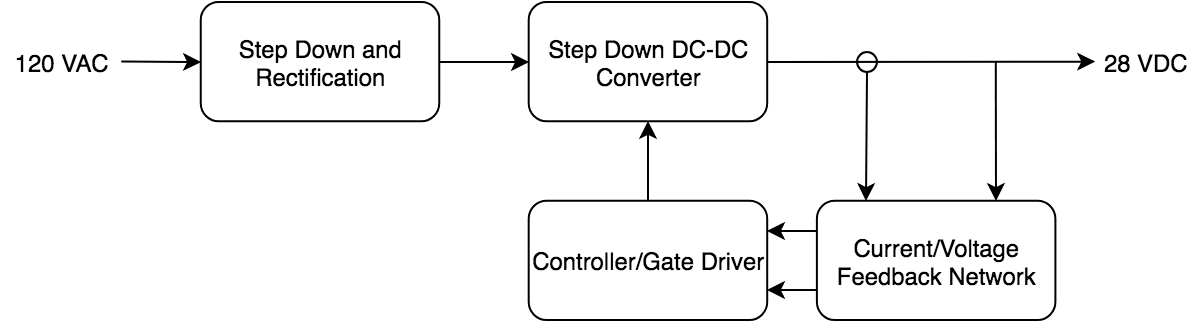
\includegraphics[scale = 0.5]{block_diagram.png}
    \caption{Functional block diagram of CSDD welder power supply.}
    \label{block}
\end{figure}

The CSDD welder power supply first takes the 120V$_{AC}$ input from a standard wall outlet. The step down and rectification block steps down the 120V$_{AC}$ to a lower AC voltage that is then rectified to a DC voltage. That voltage and is then rectified from AC to DC. This DC voltage is then input into the step down DC-DC converter stage. The DC-DC converter stage was implemented \DIFdelbegin \DIFdel{with }\DIFdelend \DIFaddbegin \DIFadd{as }\DIFaddend a variant of a buck converter. The buck converter controls the state of transistors to produce a regulated DC output. This signal is then filtered, essentially averaging the signal. The ratio between the input and output voltage of the step down DC-DC converter is ideally equal to the ratio of the "on" to the "off" times of the high side transistor. For changing load conditions this is not always the case\DIFdelbegin \DIFdel{, for }\DIFdelend \DIFaddbegin \DIFadd{. For }\DIFaddend this reason, a controller is required. The controller/gate driver block consists of a single integrated circuit (IC), the LTC3892. This IC generates \DIFdelbegin \DIFdel{an "on" time for the high side transistors to maintain }\DIFdelend the \DIFaddbegin \DIFadd{control signal driving the active components in the step down DC-DC converter to produce the }\DIFaddend desired output voltage. The controller/gate driver block \DIFaddbegin \DIFadd{IC }\DIFaddend does this using the measurements from the current/voltage feedback network. The current/voltage feedback network modifies the current and voltage measurements at the output to make them usable by the controller, as well as to provide system stability.


    \subsection{Step Down and Rectification}
        The first stage in the welder power supply is the voltage step down and AC-DC rectification. The power from 120 V$_{AC}$ mains is fed into a transformer, stepping the voltage down close to the desired output range. The stepped down AC voltage is fed into a full wave rectifier, converting the alternating current into direct current. The rectified signal is then fed into a filter composed of standard electrolytic capacitors. \DIFdelbegin \DIFdel{This }\DIFdelend \DIFaddbegin \DIFadd{The filter }\DIFaddend minimizes the voltage ripple at the output of the full wave rectifier, producing a DC voltage.

    \subsection{Step Down DC-DC Converter}
    \DIFdelbegin \DIFdel{The step down }\DIFdelend \DIFaddbegin \DIFadd{A }\DIFaddend DC-DC converter \DIFdelbegin \DIFdel{stage of the welder power supply steps down the DC voltage output of the rectifier to a level closer to the minimum contract specification. The use a DC-DC converter }\DIFdelend is necessary to ensure component failure does not occur during a short circuit at the load. DC-DC converters utilize active devices to control the voltage or current at the output. Output voltage or current regulation can be achieved when the active devices in the converter are controlled based on the conditions at the output. A standard buck topology was used to implement the step down DC-DC converter stage for several reasons. \DIFdelbegin \DIFdel{The most prominent reason that it is relatively simple}\DIFdelend \DIFaddbegin \DIFadd{A buck converter steps down a DC voltage through the use of transistors and a filter}\DIFaddend . The buck converter \DIFdelbegin \DIFdel{takes an input, turns it on and off at a }\DIFdelend \DIFaddbegin \DIFadd{disconnects and reconnects the input voltage from the filter stage at a fixed frequency and }\DIFaddend varying duty cycle\DIFdelbegin \DIFdel{, and averages it. The buck topology is also commonly used in other power supplies designed to provide power in the same current and voltage range as the CSDD }\DIFdelend \DIFaddbegin \DIFadd{. Under ideal conditions the duty cycle of the input is proportional to the output. To improve efficiency, a dual phase synchronous buck converter was used to implement this stage of the }\DIFaddend welder power supply. \DIFaddbegin \DIFadd{Dual phase essentially means that two buck converters are run in parallel. Synchronous signifies that the buck converter operates using synchronous switching, which will be elaborated on in the respective section. 
        }\DIFaddend 

    \subsection{Controller/Gate Driver}
        The controller for the \DIFdelbegin \DIFdel{welder power supply }\DIFdelend \DIFaddbegin \DIFadd{CSDD }\DIFaddend takes the information fed back from the current/voltage feedback network and controls the transistors in the DC-DC converter to produce the desired output. The controller chosen was the LTC3892. The LTC3892 uses a control architecture known as current mode control to regulate the output voltage. A controller with this control architecture was chosen because it provides inherent current limiting. Current limiting is necessary to meet the contract specification \DIFdelbegin \DIFdel{stating that }\DIFdelend \DIFaddbegin \DIFadd{that states that }\DIFaddend an output short circuit must not result in component damage. \DIFdelbegin \DIFdel{As long as the designed current limit is lower than the max rated current for each }\DIFdelend \DIFaddbegin \DIFadd{The current limit was set high enough as to not interfere with normal load current as well as not exceed the maximum rated current of the components. A safety factor was included when considering the maximum rated current }\DIFaddend of the components \DIFdelbegin \DIFdel{in the device, no component should fail during a short circuit}\DIFdelend \DIFaddbegin \DIFadd{to account for response time of the feedback system}\DIFaddend . A power transistor driver for the welder power supply is also part of the LTC3892 chip. A transistor driver is required to minimize the transition time between the transistors "on" and "off" states. The controller internally provides the "turn on" and "turn off" signals to the gate driver which subsequently changes the state of the transistors.

    \subsection{Current/Voltage Feedback Network}
        The current/voltage feedback network of the \DIFdelbegin \DIFdel{welder power supply transforms }\DIFdelend \DIFaddbegin \DIFadd{CSDD converts }\DIFaddend the output voltage and the inductor current of the DC-DC converter to voltages usable by the controller stage. The voltage at the output feeds into a voltage divider and then directly into the controller. The values of the components in the voltage divider determine the output voltage of the DC-DC converter. The controller stage compares the output of that voltage divider to a set reference voltage internally that cannot be modified by the user. A sense resistor with a known value generates a voltage proportional to the current through it. The differential voltage across the sense resistor is sent into the controller. The loop compensation network is also included in the current/voltage feedback network. The compensation network ensures stable operation of the converter to prevent undesirable oscillations at the output.

\section{Details}

\noindent This section discusses, in detail, the design of the CSDD\DIFdelbegin \DIFdel{Welder Power Supply}\DIFdelend . This includes high-level design considerations, component selection and justification, along with printed circuit board (PCB) design. This discussion is broken down into subsections on each stage included in the functional block diagram. First\DIFaddbegin \DIFadd{, }\DIFaddend the step down and rectification design \DIFdelbegin \DIFdel{will be discussed. Followed by }\DIFdelend \DIFaddbegin \DIFadd{is discussed. Next, }\DIFaddend an analysis of the step down DC-DC converter \DIFaddbegin \DIFadd{is given}\DIFaddend . The controller/MOSFET gate driver discussion comes next. \DIFdelbegin \DIFdel{Furthermore}\DIFdelend \DIFaddbegin \DIFadd{Finally}\DIFaddend , the current/voltage feedback network \DIFdelbegin \DIFdel{will then be discussedwith the details wrapping up in }\DIFdelend \DIFaddbegin \DIFadd{is discussed. The section ends with a discussion of the }\DIFaddend PCB design. 

    \subsection{Step Down and Rectification}
        The step down and rectification stage is designed to take 120V$_{AC}$ and step it down to 26V$_{AC}$ and rectify that to 36V$_{DC}$. \DIFaddbegin \DIFadd{A designed and built full wave rectifier was provided, this section overviews the verification that it would be suitable for the welder power supply. }\DIFaddend Figure \ref{fig:Full Wave Rectifier} shows the configuration of the transformer and full wave rectifier in the step down and rectification block. 

        \begin{figure}[H]
            \centering
            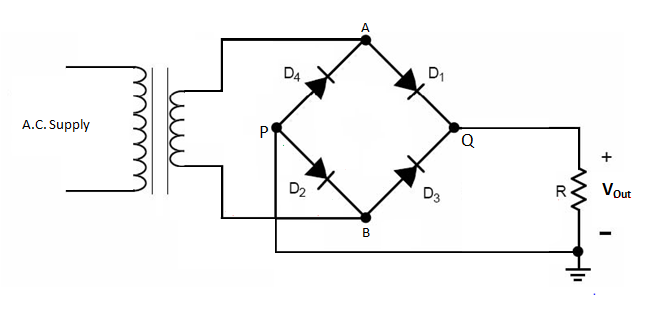
\includegraphics[width=0.5\linewidth]{fullwaverectifiercircuit.png}
            \caption{Full wave rectifier \cite{efy_group_half_207}.}
            \label{fig:Full Wave Rectifier}

        \end{figure}
         \noindent A transformer steps the 120V$_{AC}$ from mains power down to 26V$_{AC}$. \DIFdelbegin \DIFdel{A }\DIFdelend \DIFaddbegin \DIFadd{The }\DIFaddend full wave rectifier \DIFdelbegin \DIFdel{outputs a 36V$_{DC}$ from the }\DIFdelend \DIFaddbegin \DIFadd{takes the the }\DIFaddend 26V$_{AC}$ found at the output of the transformer \DIFaddbegin \DIFadd{and outputs a 36V$_{DC}$}\DIFaddend . The transformer has two independent sets of taps on the secondary winding. Each set of taps has five connections to different points on the secondary winding of the transformer. Connections to different combinations of these taps \DIFdelbegin \DIFdel{results }\DIFdelend \DIFaddbegin \DIFadd{result }\DIFaddend in different voltages at the secondary winding of the transformer. The main constraint when setting the output voltage of the step down and rectification stage is the maximum rated voltage on the smoothing capacitors. This voltage is 40V, so 26V$_{AC}$ was selected at the output of the transformer. The resulting DC output voltage of the rectifier is 36V$_{DC}$, which does not exceed the rated voltage on the smoothing capacitors.
         \newline
         \newline
         \noindent The rectifier inverts the negative component of the AC current. The resulting rectified AC signal is then fed into a large capacitor bank which filters out the majority the voltage ripple. Figure \ref{cap} shows the output of a standard full wave rectifier before and after the capacitor bank. 
         \begin{figure}[H]
            \centering
            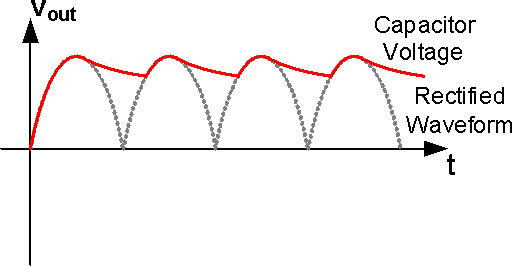
\includegraphics[width=0.6\linewidth]{2_16_0_12_eng.png}
            \caption{Rectified AC voltage filtered and unfiltered \cite{macao_communications_rectified_2012}.}
            \label{cap}
        \end{figure}
        \noindent The output voltage from the capacitor bank is used as the input for the step down DC-DC converter stage. The step down DC-DC converter design \DIFdelbegin \DIFdel{will be }\DIFdelend \DIFaddbegin \DIFadd{is }\DIFaddend presented next.

        
    \subsection{Step Down DC-DC Converter}
    The purpose of the step down DC-DC converter block is to provide output voltage regulation and current limiting. The DC-DC converter stage of the welder power supply takes the 36V$_{DC}$ output of the rectifier and steps it down to 28.6V$_{DC}$. The step down DC-DC converter stage was implemented with a type of switched mode power supply (SMPS) known as a buck converter. An example of a standard buck converter is shown in Figure \ref{buck}.

    \begin{figure}[H]
            \centering
            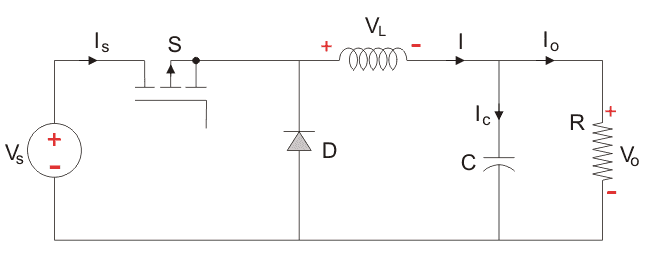
\includegraphics[width=0.6\linewidth]{1529672077.png}
            \caption{Standard buck converter \cite{electrics4u_group_standard_2019}.}
            \label{buck}
        \end{figure}

    \noindent A variety of different DC-DC converter topologies are capable of providing the necessary current at the correct voltage to meet contract specification. A boost converter was considered early on in the design process. \DIFdelbegin \DIFdel{Boost }\DIFdelend \DIFaddbegin \DIFadd{However, boost }\DIFaddend converters are inherently \DIFaddbegin \DIFadd{somewhat }\DIFaddend less efficient than buck converters \DIFdelbegin \DIFdel{. The }\DIFdelend \DIFaddbegin \DIFadd{because the }\DIFaddend inductor current of a boost converter circuit flows directly to ground during the off time of the MOSFET. Although the efficiency difference is minimal, the transformer was capable of producing a wide range of output voltage options, enabling the usage of either type of converter. \DIFdelbegin \DIFdel{From this}\DIFdelend \DIFaddbegin \DIFadd{Consequently}\DIFaddend , the design decision between the buck and boost converter \DIFaddbegin \DIFadd{was }\DIFaddend simple as the buck converter is slightly \DIFdelbegin \DIFdel{better }\DIFdelend \DIFaddbegin \DIFadd{more efficient. }\DIFaddend \cite{eric_coates_module_2018}.
    \newline
    \newline
   \noindent \DIFdelbegin \DIFdel{Another option for the Step Down DC-DC converter stage was a push-pull converter. The push-pull converter is arguably a better design choice over the buck converter for a welder power supply. Push-pull converters are widely used in high current SMPS. A schematic of a push-pull converter is shown in Figure \ref{push}.
    }%DIFDELCMD < 

%DIFDELCMD <     \begin{figure}[H]
%DIFDELCMD <             \centering
%DIFDELCMD <             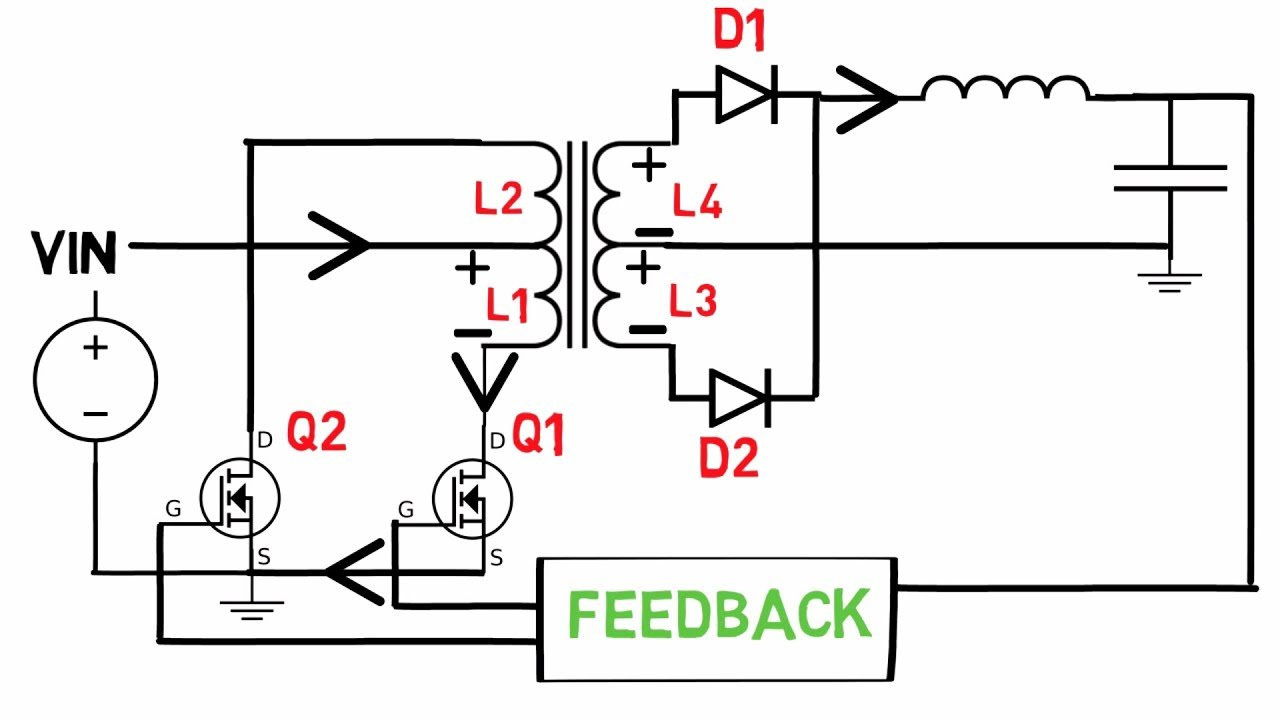
\includegraphics[width=0.5\linewidth]{maxresdefault.jpg}
%DIFDELCMD <             %%%
%DIFDELCMD < \caption{%
{%DIFAUXCMD
\DIFdelFL{Standard push-pull converter \mbox{%DIFAUXCMD
\cite{maxres_standard_nodate}}\hspace{0pt}%DIFAUXCMD
.}}
            %DIFAUXCMD
%DIFDELCMD < \label{push}
%DIFDELCMD <             

%DIFDELCMD <         \end{figure}
%DIFDELCMD <         

%DIFDELCMD <     %%%
\DIFdel{Push-pull converters produce a very steady output current on the secondary side of the transformer. This minimizes filtering necessary to produce a relatively constant output. Less filtering means a lower required capacitance and inductance, allowing the usage of smaller and possibly cheaper components. A lower output ripple current also results in lower losses that arise from the ESR of the output capacitor. The biggest disadvantage of the push-pull converter is the complicated transformer design it requires. The transformer requires 3 taps on each winding. For a high switching frequency converter, a ferrite core must be used. This makes the push-pull converter a far more expensive option for the welding power supply than a buck converter. The added efficiency along with easier inductor and capacitor selection does not warrant the added complexity and cost of the transformer design. For these reasons the buck converter was chosen as the step down DC-DC converter for the welding power supply \mbox{%DIFAUXCMD
\cite{wurth_elektronik_gmbh_&_co._switch_2019}}\hspace{0pt}%DIFAUXCMD
.
    }%DIFDELCMD < \newline
%DIFDELCMD <     \newline
%DIFDELCMD <    \noindent %%%
\DIFdel{The buck converter used to implement the CSDD welder power supply is modified slightly. The }\DIFdelend \DIFaddbegin \DIFadd{The buck converter used designed for the CSDD needed a slight modification to help with efficiency. The }\DIFaddend final converter was implemented using a dual phase synchronous buck converter. It is a synchronous buck converter because it replaces the diode in the standard topology with a MOSFET. The dual phase aspect essentially means two buck converters are run in parallel \DIFdelbegin \DIFdel{. 
   }%DIFDELCMD < \newline
%DIFDELCMD <    \newline
%DIFDELCMD <    \noindent %%%
\DIFdel{In this section, a justification for why a synchronous buck converter was used will be discussed. The dual phase buck converter section discusses the advantages of a dual phase buck converter . The component value calculations and part selection section discusses the engineering behind component selection. The current and voltage sense section overviews the measurement of the output voltage and inductor current. }\DIFdelend \DIFaddbegin \DIFadd{and out of phase. 
    }\DIFaddend 

    \subsubsection{Synchronous Buck Converter}

    \noindent  \DIFaddbegin \DIFadd{Synchronous buck converters have advantages and disadvantages over conventional buck converters. The primary advantage of a synchronous buck converter over a standard buck converter is efficiency. It is referred to as a synchronous buck converter because it is controlled through the use of synchronous switching. }\DIFaddend The standard buck converter contains two switches, one active and one passive. The active switch is usually a MOSFET, shown as the transistor in Figure \ref{buck}. The passive switch is typically a diode\DIFdelbegin \DIFdel{. In the welder power supply, the diode is }\DIFdelend \DIFaddbegin \DIFadd{, part D in Figure \ref{buck}. The  synchronous buck converter has the diode }\DIFaddend replaced with a second MOSFET.  \DIFdelbegin \DIFdel{This style of buck converter is known as a synchronous buck converter. }\DIFdelend The gate driver signals sent into each of the MOSFETs are opposite of one another. One MOSFET is on during the other's off time and vice versa. Synchronous switching in this style of converter is difficult because shoot-through current can occur if both MOSFETs are on at the same time. It essentially short circuits the input power supply through the MOSFETs. This almost always results in component damage because of the large currents that are present in short circuits. To prevent this, more complicated control circuitry is necessary in a synchronous buck converter as opposed to a standard buck converter. \DIFdelbegin \DIFdel{The main advantage of a synchronous buck converter over a standard buck converter is efficiency. }\DIFdelend Figure \ref{mosfet} is the drain to source resistance as a function of the gate to source voltage of the MOSFET used in the welder power supply. Figure \ref{diode} shows the forward current as a function of the forward voltage of a diode with voltage and current ratings comparable to the MOSFETs used the in welder power supply.

    \begin{figure}[H]
            \centering
            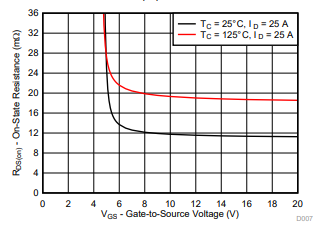
\includegraphics[width=0.5\linewidth]{mosfet.PNG}
            \caption{MOSFET (CSD18537NKCS) R$_{DS,ON}$ vs. V$_{GS}$ \cite{texas_instruments_csd18537nkcs_2013}.}
            \label{mosfet}
        \end{figure}

    \begin{figure}[H]
            \centering
            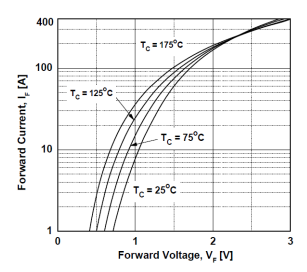
\includegraphics[width=0.5\linewidth]{diode.PNG}
            \caption{Diode (FFH60UP60S3) V$_f$ vs. I$_f$ \cite{on_semiconductor_ffh60up60s_2018}.}
            \label{diode}
             %https://www.onsemi.com/pub/Collateral/FFH60UP60S-D.PDF : done
        \end{figure}

    \noindent The voltage drop across a MOSFET when conducting 10A is on the order of 200mV when the junction temperature is 125$^{\circ}$C. A diode with a comparable current rating has a forward voltage drop of 750mV when conducting 10A at 125$^{\circ}$C. Power loss due to the resistance is equal to the voltage times the current. A higher voltage drop means more losses. Therefore a MOSFET \DIFdelbegin \DIFdel{looses }\DIFdelend \DIFaddbegin \DIFadd{loses }\DIFaddend less energy to heat when conducting than a diode. Proving that a low-side MOSFET operating in the place of a diode in a buck converter results in more efficient converter operation. 
    \DIFdelbegin \DIFdel{This advantage is typically only worth the trade-off in design difficulty for high current applications. The added design difficulty stems from the extra precautions that }\DIFdelend \DIFaddbegin \newline
    \newline
    \DIFadd{The benefits of synchronous buck converter come at the cost of increased design complexity. Added precautions }\DIFaddend must be taken to prevent shoot-through currents. \DIFaddbegin \DIFadd{These occur when both the hide side and low side MOSFETs are on at the same time, essentially short circuiting the input voltage supply. }\DIFaddend For these reasons synchronous switching is not typically implemented in low current SMPS applications \DIFaddbegin \DIFadd{as the efficiency advantage is not deemed worthwhile}\DIFaddend .

    \subsubsection{Dual Phase Buck Converter}

    \noindent A dual phase synchronous buck converter is essentially two synchronous buck converters operating in parallel. The \DIFdelbegin \DIFdel{outputs are tied together in addition to the inputs, splitting the load current between each converter}\DIFdelend \DIFaddbegin \DIFadd{load on each phase is halved as one phase can supply current during the other's off time, and  vice versa}\DIFaddend . Individual components in each phase can be smaller as a result. \DIFdelbegin \DIFdel{As stated previously, for low current applications this is not an advantage as two of each components have to be purchased. }\DIFdelend When designing a power supply capable of supplying greater than 10A of current this \DIFaddbegin \DIFadd{complicated setup }\DIFaddend is advantageous. \DIFdelbegin \DIFdel{It halves }\DIFdelend \DIFaddbegin \DIFadd{First, }\DIFaddend the necessary current rating \DIFdelbegin \DIFdel{of }\DIFdelend \DIFaddbegin \DIFadd{for }\DIFaddend the inductors in each phase \DIFdelbegin \DIFdel{. Making inductor selection easier and cheaper }\DIFdelend \DIFaddbegin \DIFadd{is cut in half. Consequently, inductor selection is easier and less expensive, }\DIFaddend as the cost of inductors increases greatly as the saturation current rating increases. Another \DIFdelbegin \DIFdel{difficulty in inductor selection }\DIFdelend \DIFaddbegin \DIFadd{problem with choosing inductors }\DIFaddend is that the inductance \DIFaddbegin \DIFadd{rating }\DIFaddend in a specific product line drops as the rated current increases. The thickness of wire\DIFaddbegin \DIFadd{, that makes up the coils of the inductor, }\DIFaddend increases as current rating increases, decreasing the number of turns a manufacturer can fit into a given inductor core. \DIFdelbegin \DIFdel{Inducatnce }\DIFdelend \DIFaddbegin \DIFadd{Inductance }\DIFaddend is proportional to the number of turns. A higher inductance allows the converter to operate at a lower switching frequency for a given ripple current. \DIFaddbegin \DIFadd{Lower switching frequency operation reduces noise pickup in traces where noise is undesirable. }\DIFaddend Therefore, a higher inductance is desirable.
    \newline
    \newline
    \noindent Another advantage the dual phase buck converter offers is input and output ripple current cancellation. This cancellation occurs because the high side MOSFETs operate 180$^{\circ}$ out of phase with each other. Figure \ref{outripple} shows the inductor ripple currents in each phase and resulting output capacitor ripple current.

    \begin{figure}[H]
            \centering
            \DIFdelbeginFL %DIFDELCMD < 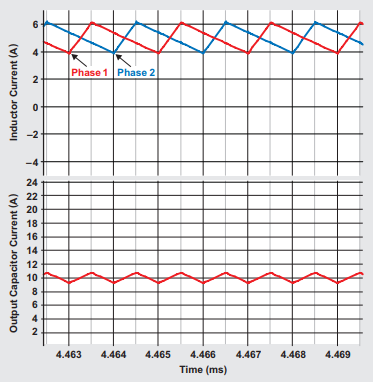
\includegraphics[width=0.4\linewidth]{outputripplecap.PNG}
%DIFDELCMD <             %%%
\DIFdelendFL \DIFaddbeginFL 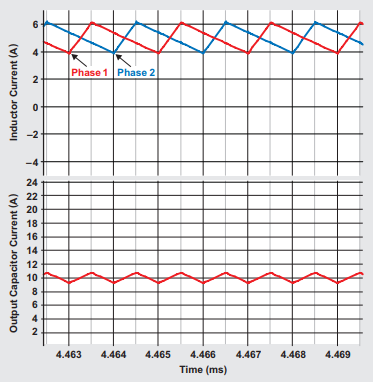
\includegraphics[width=0.5\linewidth]{outputripplecap.PNG}
            \DIFaddendFL \caption{Cancellation of the inductor ripple currents with a 25\% duty cycle \cite{david_baba_benefits_2012}.}
            \label{outripple}
             %http://www.ti.com/lit/an/slyt449/slyt449.pdf : done
        \end{figure}

    \noindent The individual inductor phase currents shown in Figure \ref{outripple} are what the output capacitor current would be if a dual phase configuration had not been used. Figure \ref{inripple} shows a plot of the normalized input RMS current as a function of the duty cycle of the converter. 

    \begin{figure}[H]
            \centering
            \DIFdelbeginFL %DIFDELCMD < 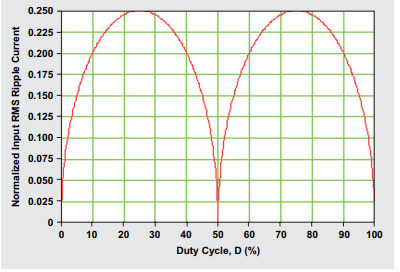
\includegraphics[width=0.4\linewidth]{inputripple.PNG}
%DIFDELCMD <             %%%
\DIFdelendFL \DIFaddbeginFL 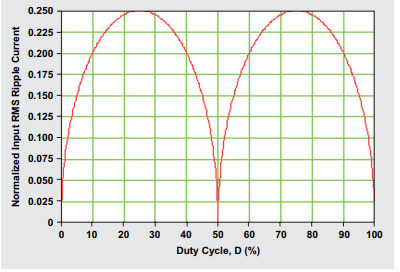
\includegraphics[width=0.5\linewidth]{inputripple.PNG}
            \DIFaddendFL \caption{Normalized inductor ripple current vs. duty cycle \cite{david_baba_benefits_2012}.}
            \label{inripple}
             %http://www.ti.com/lit/an/slyt449/slyt449.pdf : samem as previous
        \end{figure}

    \noindent The reduced inductor ripple current lessened the required amount of capacitance at the output of the \DIFdelbegin \DIFdel{welder power supply. Reducing }\DIFdelend \DIFaddbegin \DIFadd{CSDD0. This outcome reduced }\DIFaddend the required ripple current rating of both the input and the output capacitors. The input current rating of a capacitor is based on the thermal limitations of the package and the Equivalent Series Resistance (ESR) of the capacitor. The ripple current matters for converter efficiency as the capacitor sources and sinks the ripple current to maintain a relatively constant output voltage. Any time the capacitor sources or sinks current, I$^2$R losses result from the ESR of the capacitor. 

    \subsubsection{Component Value Calculations and Part Selection}
    \noindent The first component that had to be chosen for the buck converter was the \DIFdelbegin \DIFdel{inductor}\DIFdelend \DIFaddbegin \DIFadd{inductors for each phase}\DIFaddend .
    The standard inductor ripple current per phase is typically designed to be anywhere from 30\% to 70\% of the total inductor current. Equation (\ref{inductrip}) shows the equation used to calculate the inductor ripple current \cite{linear_technology_ltc3892:_nodate}.

    \begin{equation}
        i_{ripple}=(1/(f*L))*V_{OUT}*(1-V_{OUT}/V_{IN}),
        \label{inductrip}
    \end{equation}

    \noindent \DIFdelbegin \DIFdel{Where }\DIFdelend V$_{IN}$ is the output of the rectifier, 36V$_{DC}$, and V$_{OUT}$ is the desired output voltage. The two variables that can be modified in the equation are the inductor value and the switching frequency. For maximum efficiency and minimum noise the switching frequency must be as low as possible. A higher switching frequency results in the generation of higher frequency harmonics in traces with large switching currents. The impedance of a trace is proportional to frequency, a higher frequency results in a higher impedance. Therefore, voltages induced on noisy signal traces will be greater the higher the switching frequency of the converter. However, efficiency is maximized as switching frequency increases because of transition times in the MOSFETs. \DIFaddbegin \DIFadd{Minimizing noise pickup was determined to be more important than maximizing efficiency as minimizing noise is essential to proper converter operation. }\DIFaddend Switching losses in transistors occur because MOSFETs take time to transition fully between cut-off and saturation. During this transition the MOSFETs are in triode which means they are acting as variable resistors, resulting in greater I$^2$R losses. The more often the MOSFETs are turned on and off, the more losses are incurred due to switching losses. The design decision was made to minimize noise\DIFdelbegin \DIFdel{as }\DIFdelend \DIFaddbegin \DIFadd{, }\DIFaddend ensuring accurate voltage and current measurements \DIFdelbegin \DIFdel{is pertinent to converterfunction
    }\DIFdelend \DIFaddbegin \DIFadd{for a well performing converter.
    }\DIFaddend \newline
    \newline
    \noindent An inductor ripple current between 30\% and 70\% of the total output current is recommended by the data sheet for the controller \cite{linear_technology_ltc3892:_nodate}. To pick the required inductance, a ripple current of 30\%  of the desired phase current \DIFaddbegin \DIFadd{was required }\DIFaddend to meet specification. \DIFdelbegin \DIFdel{30\% }\DIFdelend \DIFaddbegin \DIFadd{Thirty percent }\DIFaddend of the phase current was chosen and not 70\% because larger capacitors are required at the output. The output capacitor ripple current would mean the desired 30\% of 15A is 4.5A, \DIFaddbegin \DIFadd{which is }\DIFaddend the desired ripple \DIFaddbegin \DIFadd{current}\DIFaddend . The chosen controller IC can operate at a switching frequency between 50kHz and 1MHz \cite{linear_technology_ltc3892:_nodate}. A switching frequency of 150kHz was selected as it resulted in a common inductance value, making inductor selection easier. The resulting inductance when calculated for this switching frequency is approximately 9.22$\mu$H. The inductor selected is the 994-SER2918H-103KL, which is manufactured by Coilcraft shown in Appendix \ref{pdf:Expense Report/Parts List}. This inductor has an inductance of 10 $\mu$ H and a maximum DC current of 28A. 10$\mu$H is reasonably close to the calculated 9.22$\mu$ H, and the 28A far exceeds the phase current required for the converter to meet contract specification \cite{noauthor_shielded_2017}.
    \newline
    % https://www.mouser.com/ProductDetail/Coilcraft/SER2918H-103KL?qs=zCSbvcPd3parQgpJIAepFA%3D%3D : done
    \newline 
    \noindent The selection of the output capacitor was the next step in designing the buck converter. The capacitance at the output affects the transient response as well as the output voltage ripple. Neither of these have specifications included in contract so they were not focused on during design. The output capacitor had to be able to maintain a capacitive impedance at frequencies at or above 150kHz. Aluminum electrolytic capacitors were ruled out as they typically look inductive above 10kHz as Figure \ref{capacitors1} shows \cite{kemet_charged_single-ended_2017}. Ceramics offer the most desirable impedance but they do not offer the bulk capacitance required to maintain the output voltage under the large load transients. Polymer capacitors seem to be the best option as they remain capacitive until 300kHz, above the switching frequency of the converter. A ceramic bypass capacitor needed to be added in parallel so that the output still looked capacitive to higher frequency resonants generated in the circuit.

    \begin{figure}[H]
            \centering
            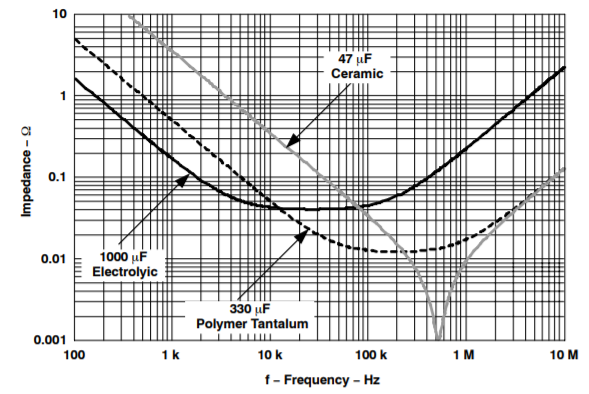
\includegraphics[width=0.5\linewidth]{capacitors.PNG}
            \caption{Impedance characteristics of different capacitors \cite{jason_arrigo_input_2006}.}
            \label{capacitors1}
             %http://www.ti.com/lit/an/slta055/slta055.pdf : done
    \end{figure}

    \noindent The other main constraint on capacitor selection is the ripple current rating. The worst case for inductor ripple current was assumed, being double the phase ripple current which is 9A. An aluminum polymer capacitor was selected to provide the bulk capacitance at the output. The aluminum polymer capacitor is the A759PY337M1JAAE042 \cite{kemet_charged_single-ended_2017}. This capacitor has a capacitance of 330$\mu$F and a ripple current rating of 4.03A @ 100kHz. Three of these capacitors placed in parallel means the collective maximum ripple current is 12.1A @ 100kHz\DIFdelbegin \DIFdel{. }\DIFdelend \DIFaddbegin \DIFadd{, }\DIFaddend 30$\%$ greater than the worst case for the ripple current experienced by the load capacitors. A standard 10 $\mu$F ceramic capacitor was placed in parallel as a bypass capacitor \cite{kemet_charged_single-ended_2017}.
    \newline
    \newline
    \noindent The next components that had to be selected for the buck converter were the transistors. The \DIFdelbegin \DIFdel{three }\DIFdelend best options for the transistors are MOSFETs \DIFdelbegin \DIFdel{, Bipolar Junction Transistors (BJTs), }\DIFdelend and Insulated Gate Bipolar Transistors (IGBTs). The decision \DIFdelbegin \DIFdel{among these three }\DIFdelend \DIFaddbegin \DIFadd{between these two }\DIFaddend types of transistors was easy as a unipolar device is necessary to implement a synchronous buck converter. This is because the current must flow from ground through the low-side transistor to the load during the off-time of the high-side transistor. \DIFdelbegin \DIFdel{BJTs and }\DIFdelend IGBTs are bipolar devices\DIFdelbegin \DIFdel{, this }\DIFdelend \DIFaddbegin \DIFadd{. This }\DIFaddend means that the device \DIFdelbegin \DIFdel{cannot conduct in any directionexcept }\DIFdelend \DIFaddbegin \DIFadd{can only conduct in one direction: }\DIFaddend from the collector to the emitter. \DIFdelbegin \DIFdel{PNP, BJTs, or IGBTs would need to be used as the emitter can be at a higher potential than the collector and the device can still function as intended. Requiring more complicated boot strapping when generating the low side gate driver voltages. For these reasons }\DIFdelend \DIFaddbegin \DIFadd{For this reason, }\DIFaddend MOSFETs were chosen as they are uni-polar devices and current can flow in either direction with no issues.
    \newline
    \newline
    \noindent The \DIFdelbegin \DIFdel{MOSFET chosen to implement }\DIFdelend \DIFaddbegin \DIFadd{transistors on the buck converter needed to be rated for at least 38V as that is the DC input voltage. They also needed to be able to withstand at least the double to phase current (10A), to account for inrush currents and delays in the feedback system. A low gate charge is also necessary in order for the controller IC's internal voltage regulator to be able to drive the MOSFET gates. The MOSFET chosen for }\DIFaddend the high-side and low-side switches in the buck converter was the CSD18537NKCS. The maximum current rating for this MOSFET is 39A at a junction temperature of 100$^{\circ}$C\DIFdelbegin \DIFdel{. Well over }\DIFdelend \DIFaddbegin \DIFadd{, well above }\DIFaddend the necessary maximum current rating to meet contract specification. The maximum V$_{DS}$ for the MOSFET is 60V\DIFdelbegin \DIFdel{, this }\DIFdelend \DIFaddbegin \DIFadd{. This }\DIFaddend is also well over any expected voltage drop across the MOSFET when it is not conducting. The advantage of this MOSFET over \DIFaddbegin \DIFadd{a }\DIFaddend MOSFET with similar I$_{DS}$ and V$_{DS}$ ratings is the low gate charge. The MOSFET gate charge as a function of V$_{GS}$ is shown in Figure \ref{mosfetgate}.

    \begin{figure}[H]
            \centering
            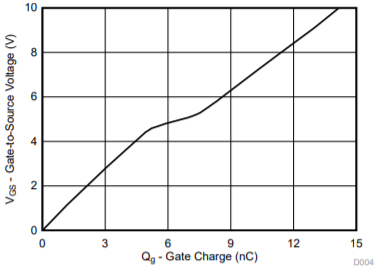
\includegraphics[width=0.5\linewidth]{mosfetgatecharge.PNG}
            \caption{MOSFET gate charge as a function of V$_{GS}$ \cite{shen_yaur_chen_block_2016}.}
            \label{mosfetgate}
             %http://www.ti.com/lit/ds/symlink/csd18537nkcs.pdf : done earlier
    \end{figure}

    The \DIFdelbegin \DIFdel{gate charge of the MOSFET determines how much current is required to bring V$_{GS}$ in a set amount of time}\DIFdelend \DIFaddbegin \DIFadd{MOSFET gate charge determines how quickly transitions between it's on/off states}\DIFaddend . A lower gate charge results in faster turn on/off times for a constant gate drive current. \DIFdelbegin \DIFdel{The }\DIFdelend \DIFaddbegin \DIFadd{Therefore, the }\DIFaddend MOSFET spends less time operating \DIFdelbegin \DIFdel{int he }\DIFdelend \DIFaddbegin \DIFadd{in the }\DIFaddend triode range. In triode the MOSFET has a much higher R$_{DS}$, which results in greater conduction losses. \DIFdelbegin \DIFdel{Device failure could even result if the power dissipation exceeds the maximum rating of the MOSFET}\DIFdelend \DIFaddbegin \DIFadd{The chance of device failure is increased with greater conduction losses as MOSFETs have a limitation on the amount of power they can dissipate}\DIFaddend .
    \newline
    \newline
    \noindent The gate driver internal to the controller IC also has a limit on how much current it can provide to the MOSFET gates. The controller data sheet provides Equation (\ref{gatedrive}) to estimate the average current sourced form the interal LDO to drive the MOSFET gates. 

    \begin{equation}
        I_{GateDrive}=2*f*(Qg_T+Qg_L),
        \label{gatedrive}
    \end{equation}
    % datasheet

    \noindent When configuring the controller\DIFaddbegin \DIFadd{, the team chose }\DIFaddend a V$_{GS}$ of 10V\DIFdelbegin \DIFdel{was chosen }\DIFdelend \DIFaddbegin \DIFadd{, }\DIFaddend as it results in the lowest R$_{DS,on}$ \DIFaddbegin \DIFadd{\mbox{%DIFAUXCMD
\cite{shen_yaur_chen_block_2016}}\hspace{0pt}%DIFAUXCMD
}\DIFaddend . The gate charge at that voltage is 14 nC. The high-side MOSFET gate charge \DIFdelbegin \DIFdel{(}\DIFdelend \DIFaddbegin \DIFadd{is represented by }\DIFaddend Qg$_T$\DIFdelbegin \DIFdel{) }\DIFdelend \DIFaddbegin \DIFadd{, }\DIFaddend and the low-side MOSFET gate charge \DIFdelbegin \DIFdel{(}\DIFdelend \DIFaddbegin \DIFadd{is represented by }\DIFaddend Qg$_L$\DIFdelbegin \DIFdel{)}\DIFdelend . The switching frequency of the controller (f) is set to 150kHz. The resulting average gate drive current is 8.4mA. The maximum average current the internal LDO for the gate drivers can provide is 50mA, which is limited to 31mA because the package chosen. Therefore, the 8.4mA necessary to drive the gates of these MOSFETs is well within the capability of controllers internal LDO.

     \subsubsection{Current and Voltage Sense}
    \noindent To enable the controller to control the output voltage and current\DIFaddbegin \DIFadd{, }\DIFaddend two feedback loops are necessary, a feedback loop for the output voltage and another for the inductor current. The controller has a set reference voltage for comparing the output. In order for the controller to regulate the output to the correct voltage\DIFaddbegin \DIFadd{, }\DIFaddend a voltage divider must be placed between the output \DIFdelbegin \DIFdel{, }\DIFdelend and the feedback pin on the controller. The values of the resistors in this feedback network were calculated using Equation \DIFdelbegin \DIFdel{\ref{vfbeq}}\DIFdelend \DIFaddbegin \DIFadd{(\ref{vfbeq})}\DIFaddend . The feedback network schematic is shown in Figure \ref{vfbpin}.

    \begin{figure} [H]
        \centering
        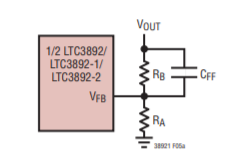
\includegraphics{vfeedback.PNG}
        \caption{Voltage feedback network. \cite{linear_technology_ltc3892:_nodate}.}
        \label{vfbpin}
    \end{figure}

    \begin{equation}
        V_{OUT} = 0.8*(1+R_B/R_A),
        \label{vfbeq}
    \end{equation}

    \noindent The desired output voltage is 28 V$_{DC}$. Using the equation the values of R$_B$ and R$_A$ were calculated to be 59.2k$\Omega$ and 1.74k$\Omega$ respectively. The feedforward capacitor C$_{FF}$ was not utilized in the voltage feedback network. Although it improves the bandwidth of the system, it negatively effects stability by decreasing the phase margin \cite{linear_technology_ltc3892:_nodate}.
    \newline
    %https://www.analog.com/media/en/technical-documentation/data-sheets/38921fc.pdf : done earlier
    \newline
    \noindent To measure the current, a sense resistor was places in series with each inductor to convert the current into a differential voltage. The voltage across this sense resistor is measured differentially by the controller. The value of the sense resistor is based on the desired current limit in each phase and current limit threshold set on the controller. The value of the current sense resistor was calculated using Equation (\ref{currentsense}).

    \begin{equation}
        R_{sense}=V_{sense,max}/(I_{max}*1.2+I_{ripple}/2),
        \label{currentsense}
    \end{equation}

    \noindent The value of I$_{max}$ is the maximum expected phase current under normal operating conditions. I$_{max}$ was determined by dividing the designed output current (30A) by the number of phases\DIFdelbegin \DIFdel{(2)}\DIFdelend , making I$_{max}$ 15A. The maximum expected current is multiplied by 1.2 to include a 20$\%$ safety factor in the current limit to ensure the short circuit current foldback feature the LTC3892 has does not activate under normal load conditions. 
    The value of V$_{sense,max}$ can be set to either 50mV, 75mV, or 100mV with the controller\DIFdelbegin \DIFdel{(1)}\DIFdelend . The value of V$_{sense,max}$ determines the maximum inductor current for which device can operate before the controller starts limiting the current. V$_{sense,max}$ was chosen to be 100mV because this allows the usage of a larger current sense resistor, which means the current feedback signal is larger in magnitude. This is beneficial because it means the controller receives a more accurate measurement as the signal is less effected by noise pickup in the PCB traces. The trade-off here is that the device is slightly less efficient because it results in larger I$^2$R losses \cite{linear_technology_ltc3892:_nodate}.
    \newline
    %https://www.analog.com/media/en/technical-documentation/data-sheets/38921fc.pdf : done earlier
    \newline
    \noindent The value of V$_{sense,max}$ also changes as the duty cycle of the converter varies. The variation of V$_{sense,max}$ is shown in Figure \ref{sensemax}.

    \begin{figure}[H]
        \centering
        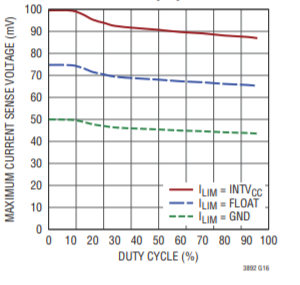
\includegraphics{vsense.PNG}
        \caption{V$_{sense,max}$ as a function of duty cycle
        \cite{linear_technology_ltc3892:_nodate}.}
        \label{sensemax}
    \end{figure}

    \noindent The average duty cycle of the device can be determined by dividing V$_{out}$ by V$_{in}$. The resulting duty cycle is about 77.8$\%$. At this duty cycle the value of V$_{sense,max}$ when set to 100mV is about 88mV. Using these values and Equation (\ref{currentsense}) the value of the current sense resistor was calculated to be approximately 4 m$\Omega$.

    \subsection{Controller/MOSFET Gate Drivers}

    \noindent The \DIFdelbegin \DIFdel{welder power supply }\DIFdelend \DIFaddbegin \DIFadd{CSDD }\DIFaddend controller was selected to be an LTC3892. According to the data sheet this controller can control a dual phase synchronous buck converter capable of providing 30A of current at 28 V$_{DC}$ \cite{linear_technology_ltc3892:_nodate}. The LTC3892 controller functions using a current mode control architecture. The standard set up for a current mode control converter is shown in Figure \ref{currentmode}. This figure shows the two feedback loops necessary to successfully implement current mode control.

    \begin{figure}[H]
        \centering
        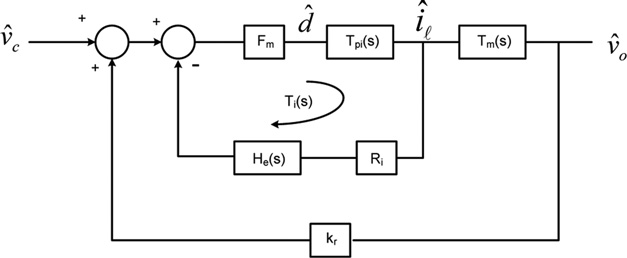
\includegraphics[width=0.5\linewidth]{Block-diagram-of-control-to-output-for-boost-converter-with-peak-current-mode-control.png}
        \caption{Current mode buck converter block diagram \cite{shen_yaur_chen_block_2016}.}
        \label{currentmode}
    \end{figure}

    \noindent A controller with a current mode control architecture was chosen mainly because it offers voltage control with built in current limiting. The voltage of the output needs to be controlled so that it remains constant over the varying load conditions one can expect when welding. The current control aspect is necessary to limit the short circuit current to ensure component damage does not occur when a short circuit is induced at the output.
    \newline
    \newline
    \noindent The controller also has an internal linear voltage regulator which it uses to provide the current to drive the gates of the MOSFETs in the buck converter. Many of the competing controllers require a separate gate driver IC specifically to drive the MOSFETs. Quite a few of the controllers that do offer internal gate drivers required a separate power supply to provide the power for the integrated gate driver. The complexity of the overall design was greatly reduced by selecting the LTC3892.

    \subsection{Current/Voltage Feedback Network}

    \noindent The current and voltage feedback network provides loop compensation for the DC-DC converter. Loop compensation is necessary in feedback control of a buck converter to ensure system stability. The first step in design the compensation network is creating a linear model for a buck converter. Creating this model is very difficult to design as the buck converter is inherently a non-linear system. A buck converter is non-linear because the MOSFETs responsible for switching are operating in non-linear regions of operation. The most simple method to model a buck converter is treating the inductor as a current source. Treating the inductor as a current source negates the effect of the LC pole generated at the output of the buck converter. The disadvantage of this model is that it is only accurate to 1/50th of the switching frequency \cite{j._li_current-mode_2009}. Such techniques are useful when designing a system that does not need to have a high bandwidth. The bandwidth is defined as the frequency at which the gain of a transfer function crosses 0 dB. The bandwidth of the system is inversely proportional to the response time for the system. The welding power supply needs to be able to respond to a short circuit at the load in far fewer than 50 cycles, making this model unusable.
    \newline
    \newline
    \noindent The buck converter was modeled using Jian Lee's model for a current mode buck converter \cite{j._li_current-mode_2009}. Jian Lee's model compared to a Simplis simulation can be seen in Figure \ref{jianlee}.

    \begin{figure}[H]
        \centering
        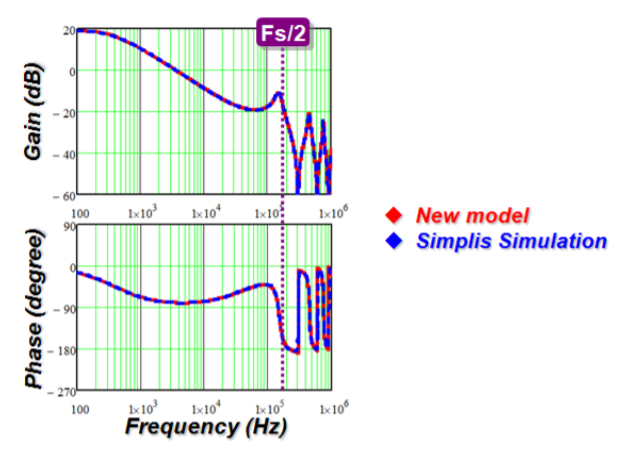
\includegraphics[width=0.7\linewidth]{controloutput.PNG}
        \caption{Control-output transfer function \cite{j._li_current-mode_2009}.}
        \label{jianlee}
    \end{figure}

    \noident The Jian Lee model for a current mode buck converter was used as G(s) in the MATLAB code in Appendix \ref{pdf:loopcompensation}. A mathematical model was created for the compensation network itself. The \DIFdelbegin \DIFdel{value of components in the compensation network were changed }\DIFdelend \DIFaddbegin \DIFadd{values of components were determined using trial and error. The values of the components in the sample designs were chosen as starting points. These values were modified }\DIFaddend until a phase margin of greater than 30$^{\circ}$ was achieved in the overall transfer function. The phase margin of 30$^{\circ}$ ensures that there is no chance that the gain will be greater than 0dB when the phase shift of the controller is 180$^{\circ}$. Meeting this condition makes the buck converter stable under various operating conditions.

    \subsection{PCB Layout}

    \noindent The PCB layout for the Welder Power Supply is crucial to the overall function of the device. High switching currents and relatively high switching \DIFdelbegin \DIFdel{frequency leads }\DIFdelend \DIFaddbegin \DIFadd{frequencies lead }\DIFaddend to noise pickup on signal traces, complicating the design of this PCB greatly. The final PCB layout of the of the Welder Power Supply is shown in Figure \ref{pcb}.

    \begin{figure}[H]
        \centering
        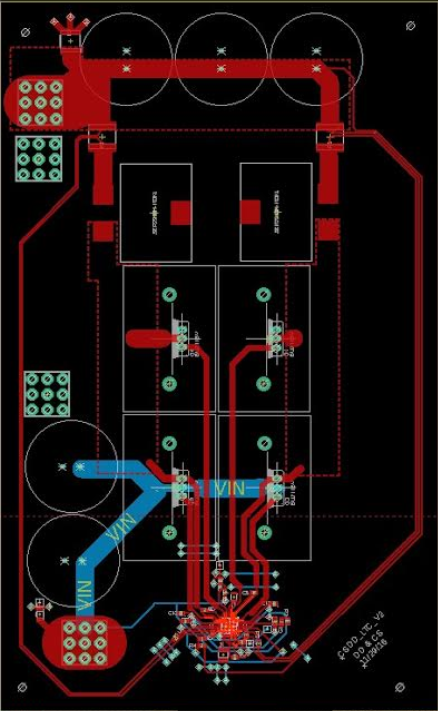
\includegraphics[width=0.3\linewidth]{pcblayout.PNG}
        \caption{Welder power supply PCB layout.}
        \label{pcb}
    \end{figure}

    \noindent The LTC3892's data sheet provided a list of conditions for the PCB layout that had to be met to get maximum performance out of the converter \cite{linear_technology_ltc3892:_nodate}. The IC and signal traces had to be kept as far away as possible from the switch node between the inductor and the high side MOSFETs. Both the current sense and voltage feedback traces had to be run by the switch node to reach the sense resistors and the output. They were run as far away as the board size would allow. The traces from each side of the sense resistors were run as close to each other as possible. Therefore, whatever noise gets picked up by one of the sense traces will get picked up by the other one as well. From this, only the common mode voltage of the traces will be effected, not the differential voltage. The differential voltage is how the signal is measured so any change to the common mode voltage has no effect on the measurement of the inductor current, making this a viable method for dealing with noise.  
    \newline
    \newline
    \noindent The tracers from the controller to the gates of each of the MOSFETs also had to be made as short as possible. Accomplishing this was a challenge as the selected heat sinks for the MOSFETs were quite large which limited how close the MOSFETs could physically be to one another. The gate driver traces ended up being short enough in order for the power supply to function.

\section{Results}
    After completing the hardware assembly, testing confirmed that the contract specifications were met. Wall outlet AC power was the only input for the entire system\DIFdelbegin \DIFdel{, }\DIFdelend \DIFaddbegin \DIFadd{; }\DIFaddend no power supplies were used. The circuit supplied at least 10A of current with a minimum of 24V$_{DC}$ at the output. In addition to the minimum output specifications\DIFaddbegin \DIFadd{, }\DIFaddend the circuit was required to function \DIFdelbegin \DIFdel{correct }\DIFdelend \DIFaddbegin \DIFadd{correctly }\DIFaddend after a short circuit was induced at the output. All data was measured using a series of multimeters and oscilloscopes \DIFdelbegin \DIFdel{that will be }\DIFdelend discussed below in their relevant sections. The power supply step down and regulation \DIFdelbegin \DIFdel{will be }\DIFdelend \DIFaddbegin \DIFadd{are }\DIFaddend discussed first, followed by the DC-DC voltage regulation, with the short circuit performance being discussed last. 

    \subsection{Power Supply Step Down and Rectification}
    The power supply step down and rectification stages were both tested with multimeters. The largest problems that came out of this section were with the input to the transformer as a result of poor connections. The wire used to connect the transformer to the wall outlet was old and began to degrade under the constant movement of the device from multiple locations. This issue led to a break in the wire that \DIFdelbegin \DIFdel{would cause }\DIFdelend \DIFaddbegin \DIFadd{caused }\DIFaddend a loss in power intermittently. After a series of tests on both the transformer and the rectifier, the wire was determined to be the problem. After replacing the wire there was no further issues with this section of the project. Testing this project required use of a multimeter that possessed both an AC and DC voltage measurement capability. The Sparkfun Electronics VC830L \DIFdelbegin \DIFdel{digital multimeter }\DIFdelend \DIFaddbegin \DIFadd{Digital Multimeter }\DIFaddend (DMM) was used to capture data. The DMM was used to measure the AC voltage before and after the transformer to check the step down function of the transformer. The input taps of the transformer measured 120V$_{AC}$, and the output of the transformer measured 26V$_{AC}$. The transformer stepped down the 120V$_{AC}$ correctly and that signal was immediately rectified. The DMM was used to check for function of the rectifier.

    This DMM was then set to measure DC voltage. The DC voltage at the output of the rectifier was expected to be 36V$_{DC}$. The output of the rectifier was precisely 36V$_{DC}$. The 36V$_{DC}$ output of the rectification circuit completed the step down and rectification section with expected results. The rectifier output was then introduced to the DC-DC voltage regulation portion of this project. 

        
    \subsection{DC-DC Voltage Regulation}
       The DC-DC voltage regulation of this welder power supply was done through the creation of a PCB with a collection of components. A large concern for this section of the project was any noise between traces. Such issues were addressed in the design of the PCB with careful placement, size, and routing of the these traces to every aspect of the board. One issue that the engineering and design \DIFdelbegin \DIFdel{crew }\DIFdelend \DIFaddbegin \DIFadd{team }\DIFaddend experienced during testing was with a trace feeding the drain of both high side MOSFETS. The largest trace that could be created in that area was not enough to handle the current that was drawn through that trace. To counter that issue, external wires were added along the PCB traces to reduce the current density. 

       Performance of the board was tested in multiple stages with different loads. The board was required to regulate a voltage above 24V$_{DC}$ under different loads. The designed voltage for this PCB to regulate was 28V$_{DC}$. The first test of voltage regulation was done with no load at the output and measurement with the DMM. The output of the PCB voltage regulator was 28V$_{DC}$, indicating that the voltage regulator was working under no load. The next step in testing the device resulted in the addition of a load to the output. The load added to the device to achieve the minimum 10A current draw was 2.6$\ohm$. The load that best fit \DIFdelbegin \DIFdel{our }\DIFdelend \DIFaddbegin \DIFadd{the }\DIFaddend application was nichrome wire. The nichrome wire can withstand a large amount of heat without breaking down while maintaining a relatively constant resistance, making it useful in testing the function of this welder power supply. A section of nichrome wire was measure with the DMM for the correct resistance then connected to the output of the project. The current for this project was measure and checked with two different devices. A Voltcraft VC330 Current Clamp Meter was place over one lead at the output and displays the current through that lead. In addition to the clamp meter, the DMM was place across the load to measure the voltage and with the resistance known between the leads, the current can be calculated. 

       With this load connected the CSDD welder power supply was turned on and the voltage at the output remained a consistent 28V$_{DC}$ with a the current measured at 11A. 

    \subsection{Short Circuit Performance}
        Testing the short circuit conditions at the output followed the same testing technique as at the introduction of load. The short circuit condition was created by touching the output leads of the power supply together. It was expected that the output current would drop to approximately 40\% of the programmed current limit, making the expected output current approximately 13A. Upon the introduction of short circuit condition, the output current dropped to approximately 12.4A. The short circuit condition was taken away and the output voltage of the welder returned to 28V$_{DC}$. This is indicative of a properly functioning power supply, proving that the short circuit condition did not cause component damage.

\section{Conclusion}

    To conclude, the project was a success and met all the specifications outlined in the contract. The CSDD welder power supply design, test, and results of the CSDD were discussed. Although the design portion and testing was very complicated, the project functioned as required. The complete project consisted of a transformer, input and output capacitors, and a complete PCB board. This welder power supply is an adaptable and unique device to power any 28V$_{DC}$ and 10A stick welding machine\DIFaddbegin \DIFadd{. 
    }

    \DIFadd{This project was inherently difficult for a multitude of reasons that came back to the high switching frequencies and currents present in the PCB. Prototyping this project was not possible from the switching frequency and currents present. In addition to the inability to prototype, designing the PCB to accommodate all the requirements and keep the noisy signals from interfering took a very long time and effort. Overall, this project was possible but the time span did not allow for as much research and design necessary to improve the CSDD to its utmost abilities}\DIFaddend . 

\newpage

\printbibliography

\newpage
\appendix
\appendixpage
\addapptotoc
\begin{minipage}[t]{0.7\linewidth}
  
\includepdf[pages=1,scale=.7,pagecommand={\section{Contract}\label{pdf:Contract}},linktodoc=true]{Contract.pdf}
\end{minipage}

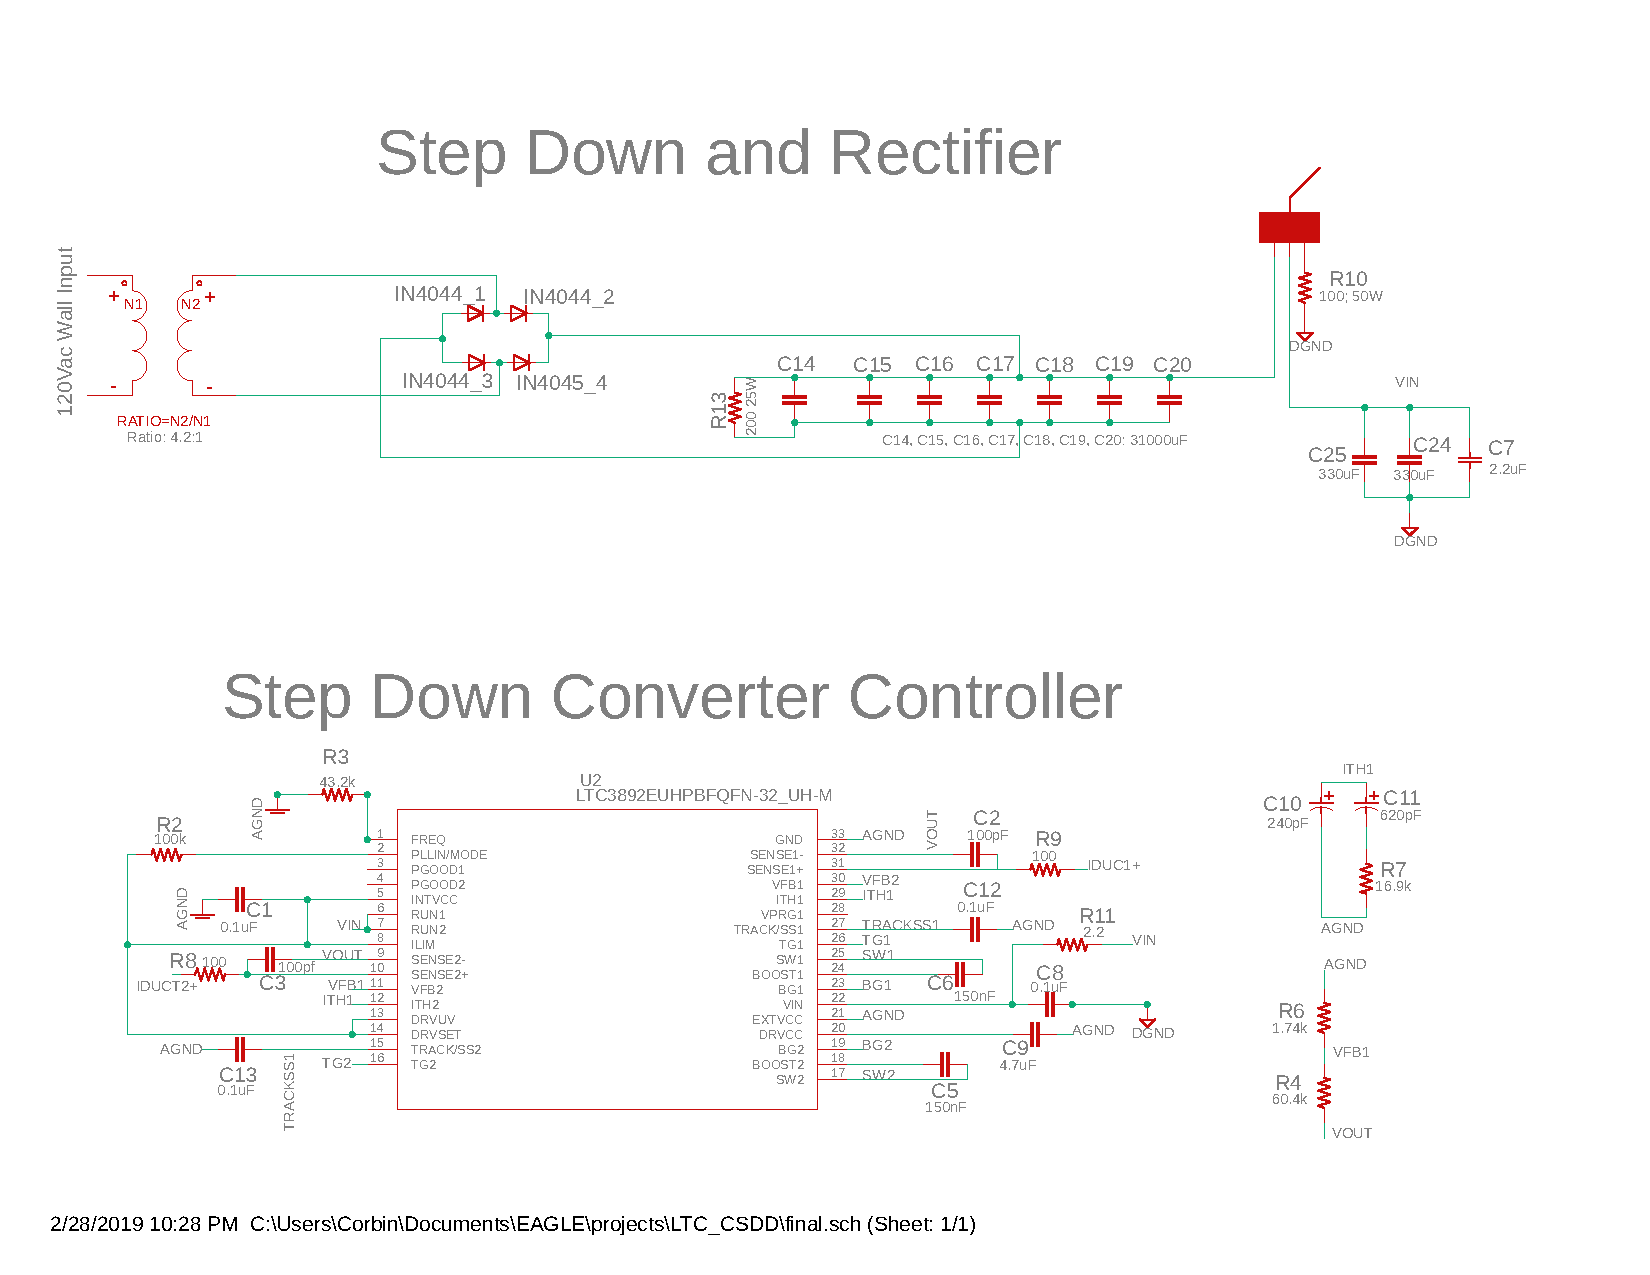
\includepdf[pages=1,scale=1,pagecommand={\section{Schematics}\label{pdf:Schematic}},linktodoc=true]{Final_Schematic.pdf}

\includepdf[pages=2-,scale=1,pagecommand={}]{Final_Schematic.pdf}

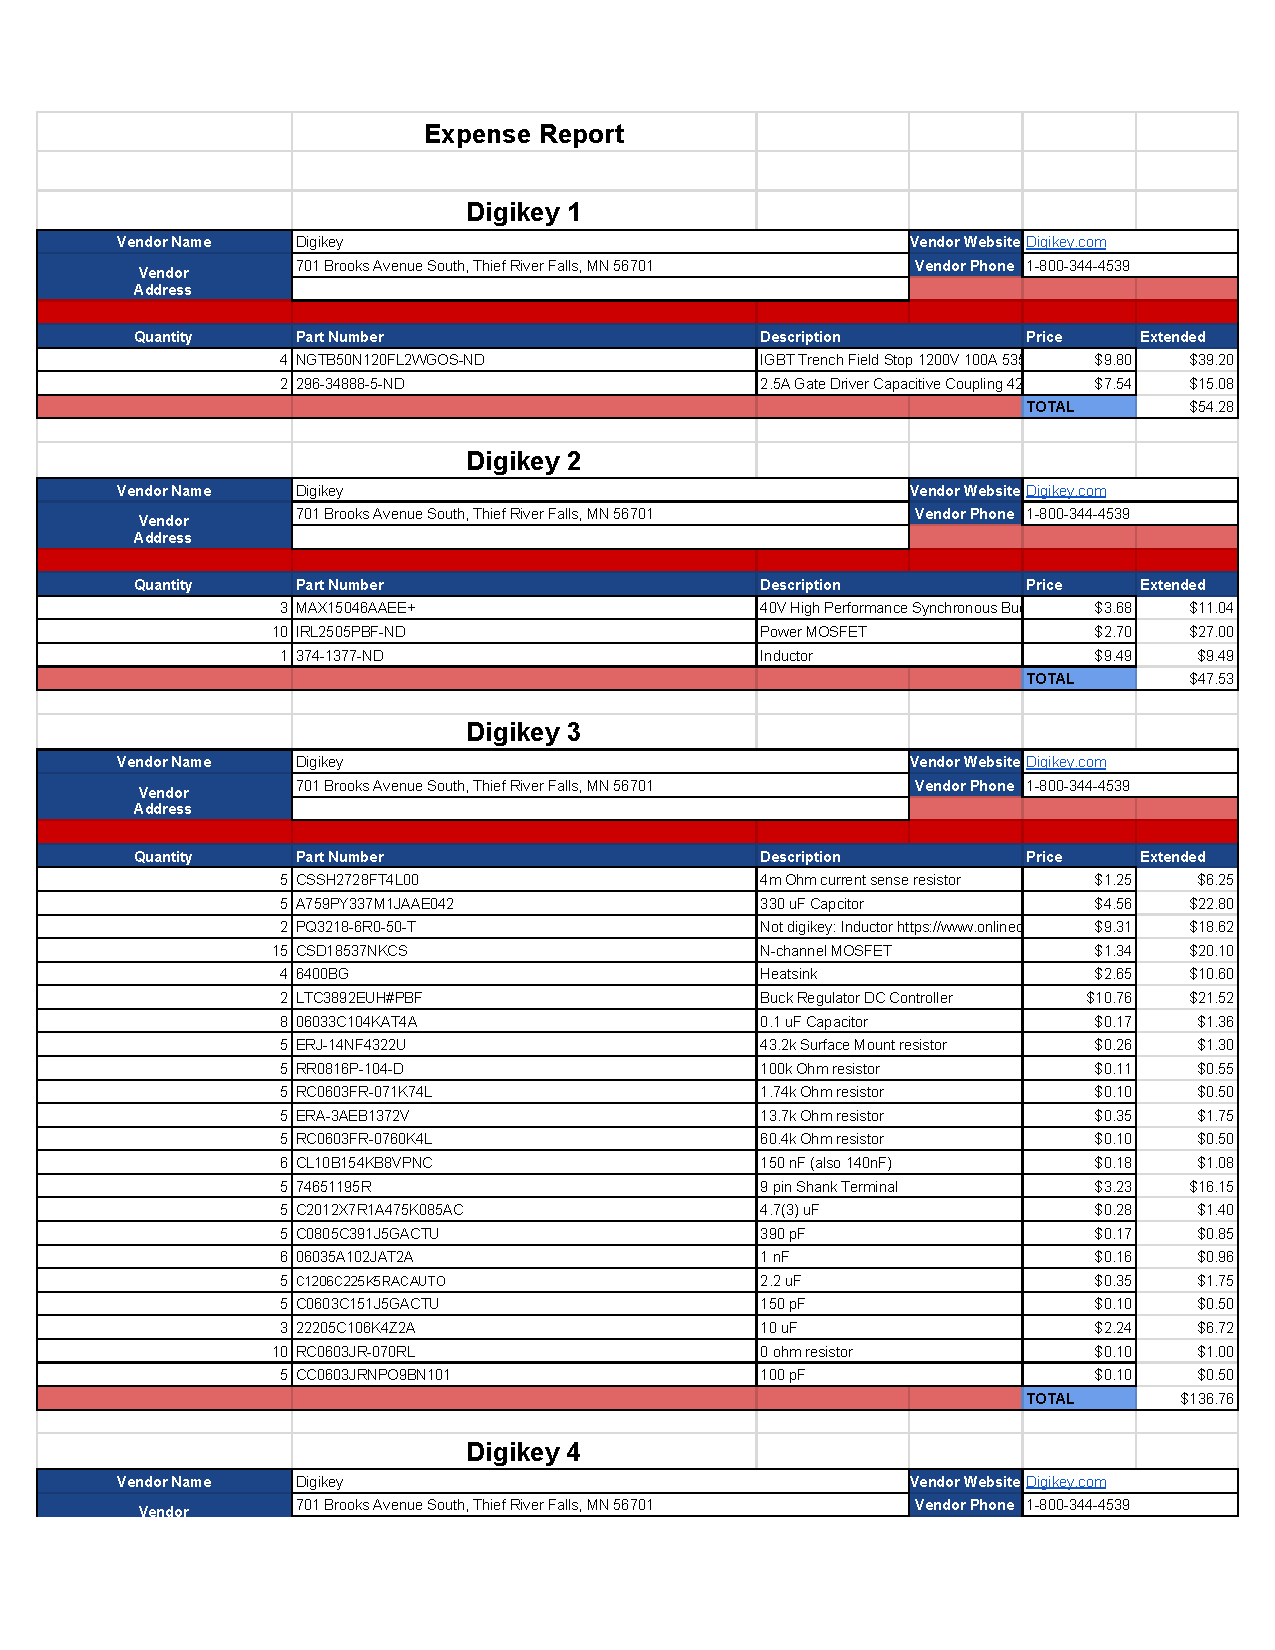
\includepdf[pages=1,scale=.8,pagecommand={\section{Parts List}\label{pdf:Expense Report/Parts List}},linktodoc=true]{ExpenseReport.pdf}

\includepdf[pages=2-,scale=.8,pagecommand={}]{ExpenseReport.pdf}

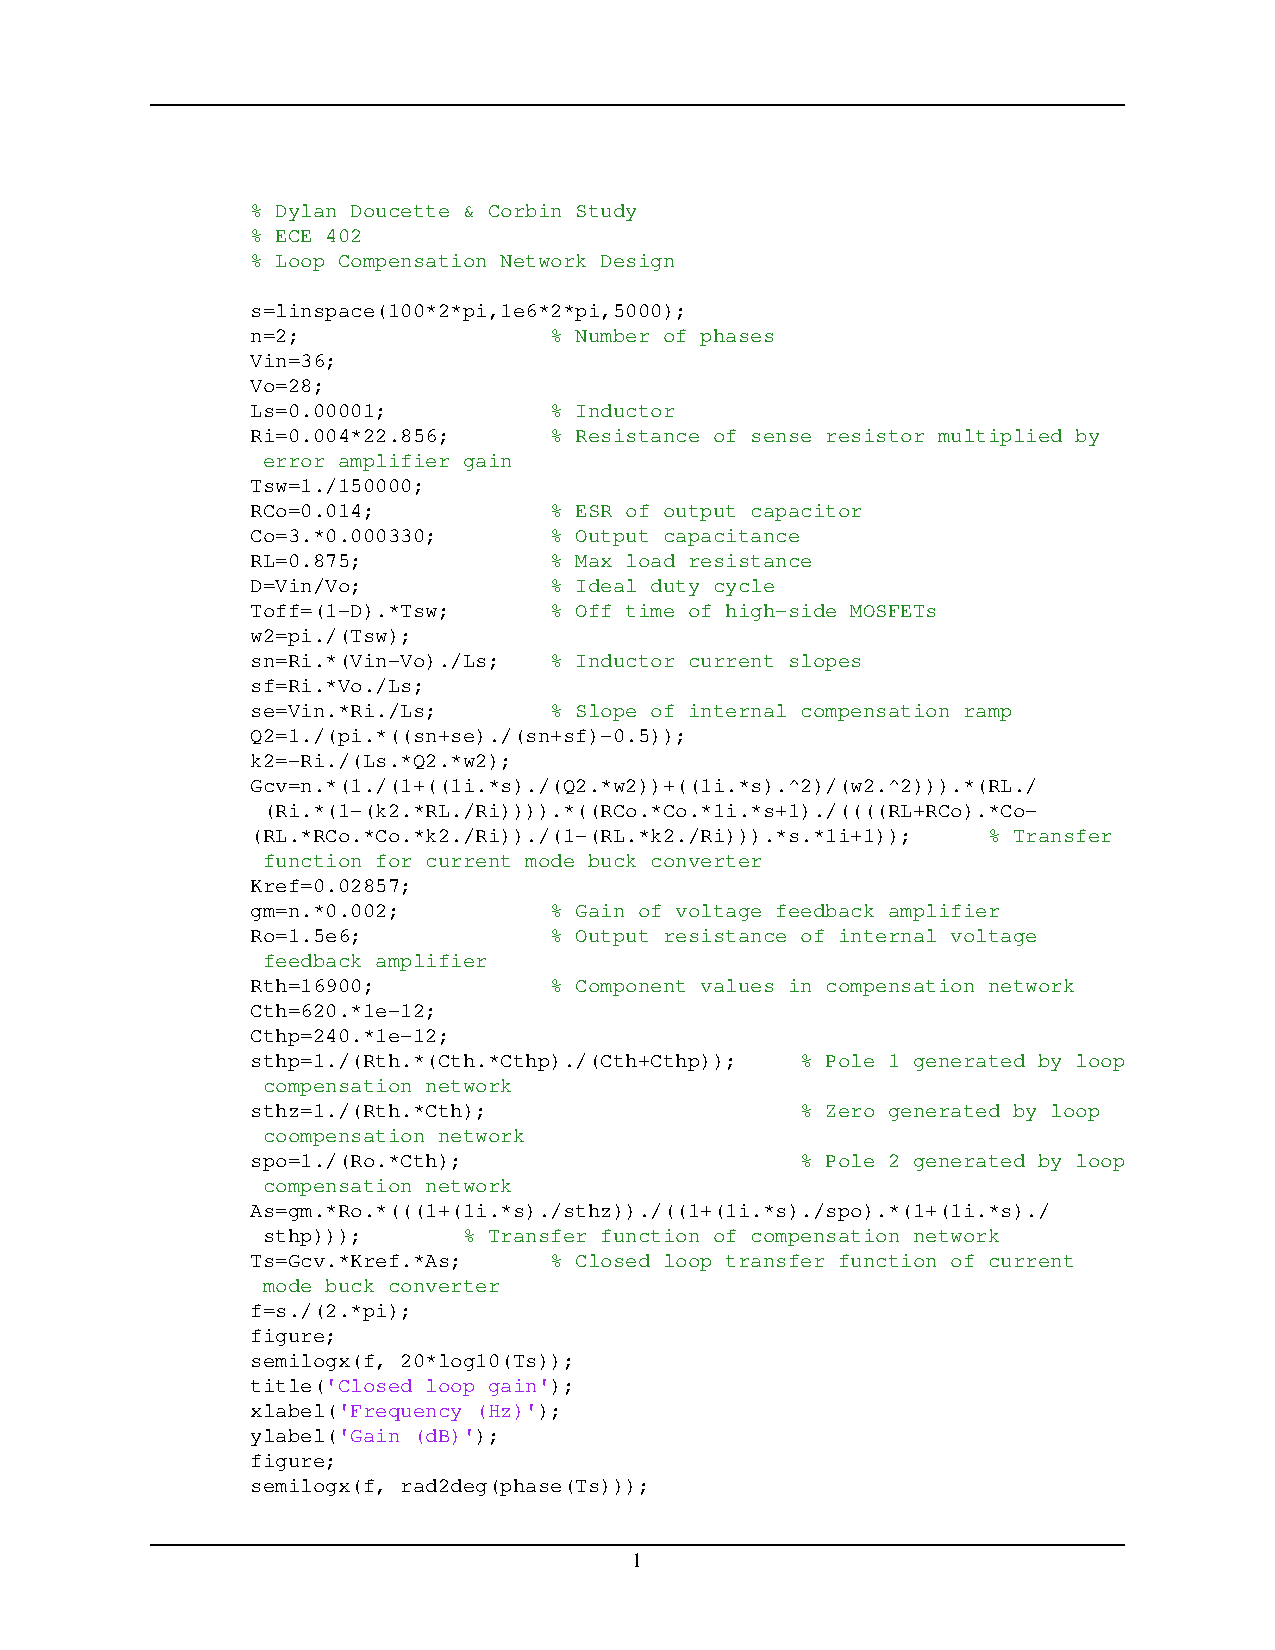
\includepdf[pages=1,scale=.8,pagecommand={\section{Loop Compensation Network Design}\label{pdf:loopcompensation}},linktodoc=true]{ece402_loopcompensation.pdf}

\includepdf[pages=2-,scale=.8,pagecommand={}]{ece402_loopcompensation.pdf}

\end{document}